\documentclass{article}
\usepackage{booktabs}
\usepackage{stfloats}
\usepackage{amsfonts}
\usepackage[fleqn]{amsmath}
\documentclass{llncs}
\usepackage{subcaption}
\usepackage[T1]{fontenc}
\usepackage{graphicx}
\usepackage{authblk}
\usepackage{etoolbox}
\makeatletter
\patchcmd{\thebibliography}
  {\clubpenalty4000\@clubpenalty\clubpenalty}
  {\clubpenalty4000\@clubpenalty\clubpenalty\setlength{\itemindent}{-2em}\setlength{\leftmargin}{2em}}{}{}
\makeatother



\begin{document}
\begin{center}
    {\LARGE {AEIN: Attention-Enhanced Iterative Join Graph Neural Networks}} \\[1.5em]
    Jixin Zhang\textsuperscript{a}, Y.Lai\textsuperscript{b} \\[0.5em]
    {\small \textsuperscript{a,b}\textit{Key Labroatory of Symbolic Computation and Knowledge Engineering 
    of Ministry of Education, Jilin University, Changchun, 130012, China}}
\end{center}

\begin{abstract}
We propose an Attention-Enhanced Iterative Join Graph Neural Networks(AEIN) model for solving \#SAT problems, 
which significantly improves the solving accuracy. Inspired by the Iterative Join Graph Propagation (IJGP) 
algorithm, AEIN uses tree decomposition to encode the CNF formula into a connection graph, then performs iterative 
message passing on the join-graph, and finally approximates the model number by learning partition functions. 
In order to further improve the accuracy of the solution, we apply the attention mechanism in and between clusters 
of the join-graphs, which makes AEIN pay more attention to the key variables and clusters in probabilistic inference, 
and reduces the redundant calculation. Finally, our experiments show that our AEIN model achieves better results 
than other neural network methods.
\end{abstract}


The propositional model counting problem \#SAT, which is the problem of calculating a satisfactory assigned quantity for a given Boolean formula, has applications including software verification\cite{A1}\cite{A2}, hardware design and planning\cite{B1}\cite{B2}\\ \cite{A3}, and is a fundamental challenge in computer science. However, \#SAT is \#P-complete and is therefore at least as computationally difficult as the NP-complete problem. Traditional exact \#SAT solvers (e.g., DPLL-based)\cite{A4}\cite{A5} struggle with large-scale CNF formulas due to exponential complexity. While approximate methods (e.g., MiniCount-based)\cite{A6} scale better, they often fail to capture complex clause-variable dependencies, leading to significant errors in structured instances, so many approximate solvers (i.e. methods that provide an estimate of the number of solutions) have been developed, which can be scaled up to larger problem sizes, but the approximate methods sacrifice a certain degree of accuracy.\\
With the superior learning capabilities of neural networks, various machine learning and deep learning methods have recently been proposed for propositional model counting problems\cite{A7}\cite{B3}\cite{B4}. A series of studies aimed at constructing independent neural solvers to solve combinatorial and logical reasoning tasks that directly predict the number of satisfactory assignments for a given instance\cite{A8}\cite{A9}. Other methods integrate neural modules into classical solvers, improving the branch heuristic algorithm in the \#SAT solver\cite{A10}. Although neural network methods show great potential to solve \#SAT, they still face some challenges. Existing GNN models (such as NSNet\cite{A11}, BPNN\cite{A12}) rely on simple belief propagation (BP) and cannot effectively model higher-order dependencies and global constraint structures between variables. Furthermore, how to combine the deep learning model with the strict reasoning of symbolic logic while ensuring that the deep learning model has good expressiveness?\cite{A12} How to enhance the reasoning ability of the model for complex constraints?\cite{A14}\\
In order to solve these problems, we propose the AEIN model in this paper. In this work, AEIN bridges the neural-symbolic gap by integrating the Iterative Join Graph Propagation  algorithm (IJGP)\cite{A15} into GNNs.   Specifically, we use GAT layers to simulate IJGP's belief updates, while tree decomposition guides hierarchical attention (intra-cluster and inter-cluster message passing). Inspired by HAN(Zichao Yang et al.,2016)\cite{B5}, this hierarchical attention method is a text classification model in which attention mechanisms are applied in layers of text. At the same time, in order to reduce the extra overhead brought by the attention mechanism, we adopt the method of dynamic pruning attention heads with the time step\cite{B6}\cite{A16}, which has more attention heads at the early stage of iteration and reduces them successively to avoid redundant calculations. As a focus of this paper, the constraint-aware attention mechanism encourages variable values to tend to satisfy clauses by showing modeling constraints (calculating attention scores) as regularization terms in the loss function, guiding the first two kinds of attention simultaneously. \\
The partition function has been shown to be a good approximation of the number of Boolean formula solutions\cite{A17}\cite{A18}, and our model similarly follows this computational approach, with careful and extensive experimental investigation, and experiments on BIRD and SATLIB benchmarks show that our method is significantly superior to NSNet. 
\textbf{Satisfiability Problems.\\} 
In propositional logic, a Boolean formula consists of Boolean variables and logical operators such as negations (¬), conjunctions ($ \land $), and disjunctions ($\lor$). It is typical to represent Boolean formulas in conjunctive normal form (CNF), expressed as a conjunction of clauses, each of which is a disjunction of literals (a variable or its negation). Given a CNF formula, the SAT problem asks whether there exists an assignment to its variables that can satisfy the formula, while the goal of \#SAT is to count the number of all satisfying solutions.\\
\textbf{Iterative Join Graph Propagation.\\}
IJGP (Iterative Join Graph Propagation) is an approximate inference algorithm primarily used to solve marginal probability computation problems in probabilistic graphical models (such as Markov Random Fields and Bayesian Networks). It constructs a Join Graph and iteratively propagates messages on the graph to achieve efficient calculation of complex probability distributions.
Given a probabilistic graphical model, its joint probability distribution can be expressed as a product of factors:
\begin{equation}
P(X)=\left(\frac{1}{Z}\right)\prod\limits_{i=1}\limits^m\phi_i(C_i)
\end{equation}
where \(\phi_i(C_i)\) is a factor defined on a subset of variables \(C_i\subseteq X\), and
\(\textbf{\textit{Z}}\) is the normalization constant (partition function).
A Join Graph is a structure that decomposes the factor graph into multiple clusters, where each cluster contains a set of variables and their associated factors. The Join Graph satisfies the following properties:\\
Coverage: Each factor \(\phi_i\) must be included in at least one cluster.\\
Connectivity: For any two clusters that share a variable, there exists a path connecting them, and all clusters on the path contain the variable.\\
The join graph in this paper was completed using the external tree decomposition tool flow-cutter, and the tree-width was manually controlled.
In the Join Graph, a message is a function sent from a cluster \(C_i\) to another cluster \(C_j\), defined as:
\begin{equation}
m_{i\rightarrow j}(S_{ij})=\sum\limits_{C_i\textbackslash S_{ij}}\phi_i(C_i)\prod\limits_{k\in ne(i)\textbackslash j}m_{k\rightarrow i}(S_{ki})
\end{equation}
\(S_{ij}=C_i\bigcap C_j\) is the set of shared variables between clusters \(C_i\) and \(C_j\),  \(ne(i)\) is the set of neightboring cluster of \(C_i\) and \(\sum\limits_{C_i\textbackslash S_{ij}}\) denotes summation over variables in \(C_i\textbackslash S_{ij}\).
The core of the IJGP algorithm is to approximate marginal probabilities by iteratively propagating messages. The specific steps are as follows:Initialize all messages \(m_{i\rightarrow j}\) to uniform distributions,For each cluster \(C_i\), compute the message sent to its neighbor \(C_j\), then, Update messages until convergence or the maximum number of iterations is reached, finally, for each variable X, the marginal probability is the product of all related messages in the clusters containing X:
\begin{equation}
P(X)\propto\prod\limits_{X\in C_i}m_{i\rightarrow j}(S_{ij})
\end{equation}
\textbf{Graph Attention Networks.}\\
The Graph Attention Mechanism (GAT) is a graph neural network model based on attention mechanisms. It dynamically aggregates information from neighboring nodes by computing attention weights between nodes.
For a node v and its neighboe \(u \in N(v)\), the attention weight \(\alpha_{vu}\) is defined as:
\begin{equation}
\alpha_{vu}=\frac{exp(LeakyReLU(a^T[Wh_v\mid\mid Wh_u]))}{\sum\limits_{k\in N(v)}exp(LeakyReLU(a^T[Wh_v\mid\mid Wh_k]))}
\end{equation}
where \(W\in \mathbb{R}^{d'\times d}\) a learnable weight matrix;\(a\in \mathbb{R}^{2d'}\) is a learnable attention vector; \(\mid\mid\) denotes vector concatenation; 
The updated representation \(h'_v\) of nodem v is obtained by weighted aggregation of information from neighboring nodes:
\begin{equation}
h'_v=\sigma(\sum\limits_{u\in N(v)}\alpha_{vu} Wh_u)
\end{equation}

\begin{figure}[h]
\centering 
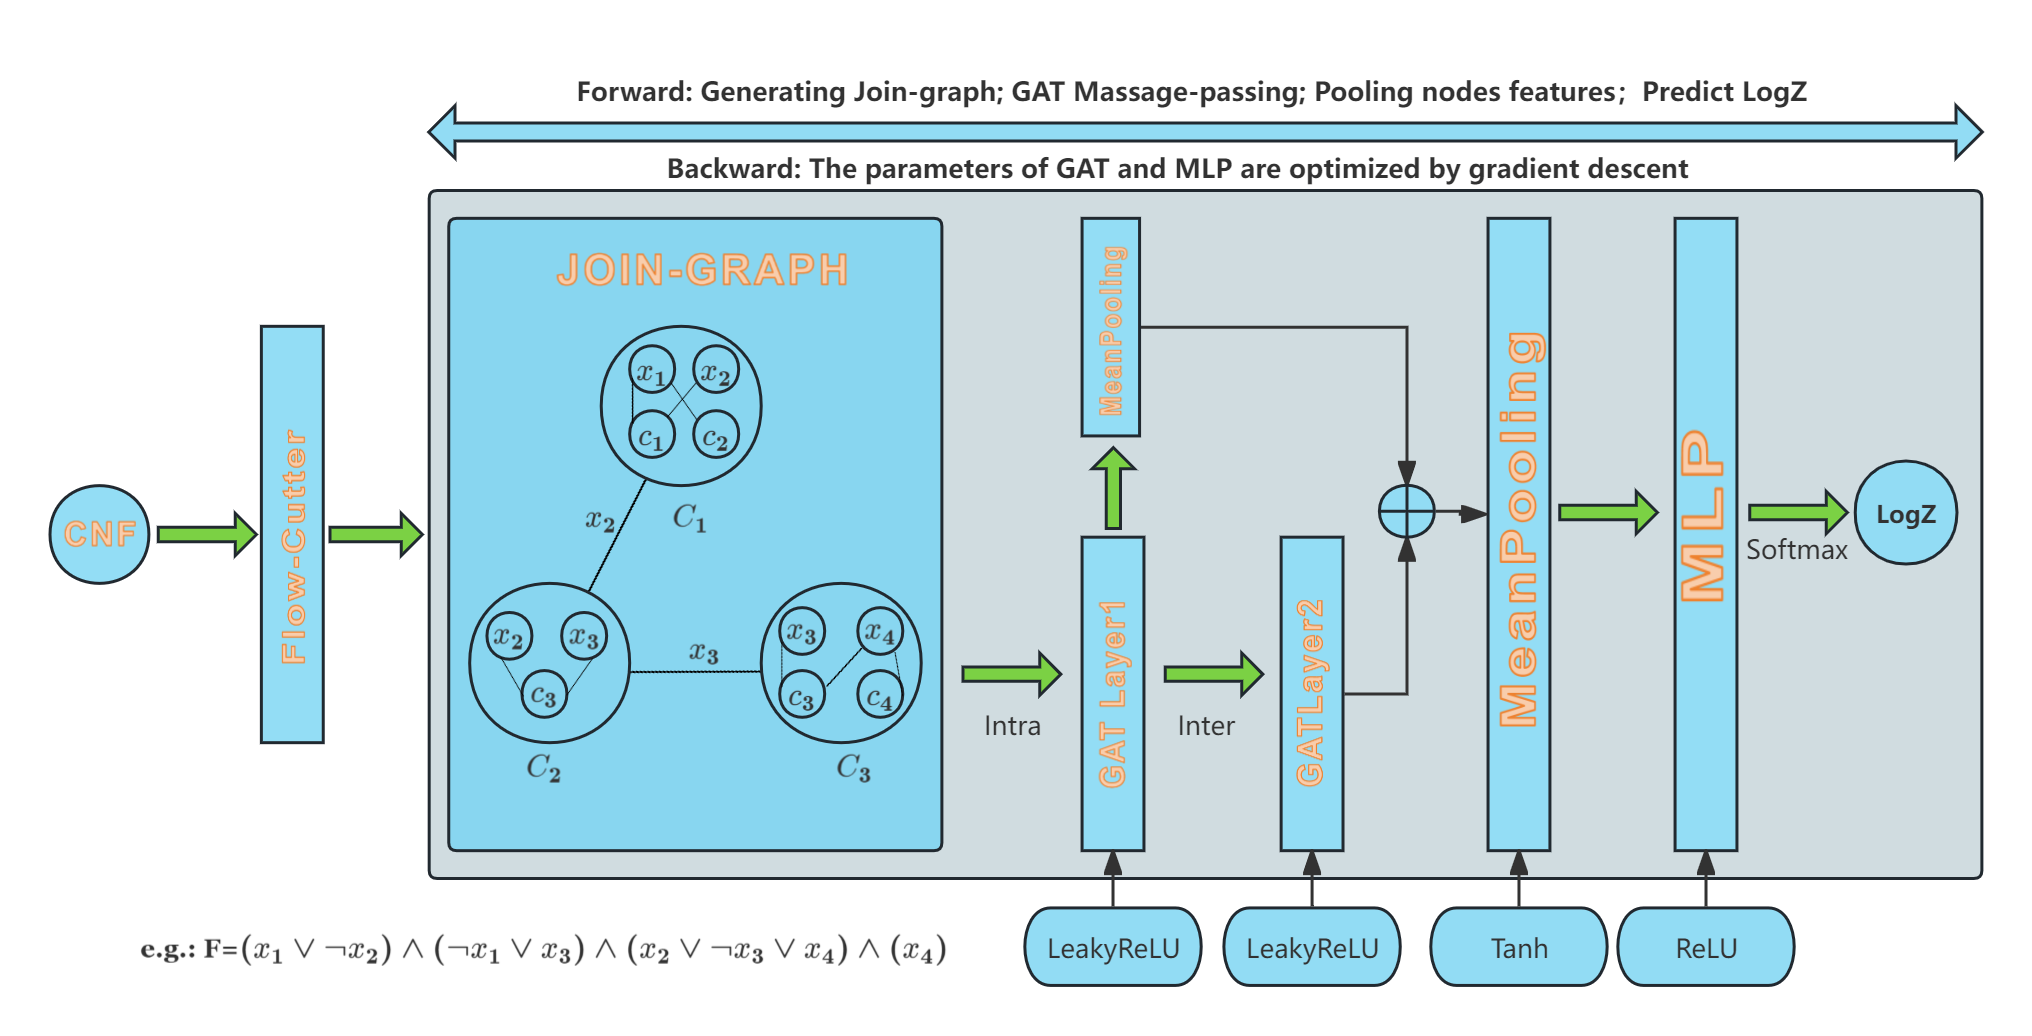
\includegraphics[width=1\textwidth]{png/AEIN2.png}
\caption{For the \#SAT problem, we use 2 GAT layers for message passing, and finally use the MLP 
layer estimated partition function as an approximate solver. The pooled layer is used to compress 
the processed variable and clause node features into a global representation that is provided to 
the MLP layer.} 
\label{fig1}
\end{figure}
In this section, we first explain our model framework and its operating principle, and then introduce 
the combination of tree decomposition and attention mechanism. This framework, as a neural version of 
IJGP, has a unique tree decomposition structure to better fit the attention mechanism. By expressing 
\#SAT as a probabilistic inference task, we show how AEIN can be used to solve this problem. (see Fig.~\ref{fig1}).

\subsection{AEIN Framework}
For a given CNF formula, we encode it in the form of a factor graph (the variable \(x_i\) has an 
edge between \(x_i\) and \(C_i\) if it is in the \(C_i\) clause), and then call an external tree 
decomposition tool to decompose the factor graph into a connection graph, generated clustering set 
\{\(C_1\), \ \(C_2\), \ldots \(C_k\)\}, each cluster contains variables and clauses of local structure 
(see figure \ref{fig2}). And initialize its variable node feature \(h_v\) and self-identifying node 
feature \(h_\phi\) in the input layer. The main architecture of the model consists of two GAT layers, 
one MLP layer, and one pooling layer. \(GAT1\) and \(GAT2\) are cyclically invoked during message 
until convergence. \(GAT1\) is responsible for local variation-clause message passing, \(GAT2\) 
is responsible for cross-cluster message passing, and aggregates messages through splicing-pooling 
operation. Finally, \(b_i(C_i)\) and \(b_i(x_i)\) are estimated by the MLP layer to output the final 
number of models. The design of the architecture is in line with the iterative nature of the IJGP 
algorithm, that is, local first, then global, and the results within a cluster directly affect the 
propagation weight between clusters.
\begin{figure}[h]
\centering 
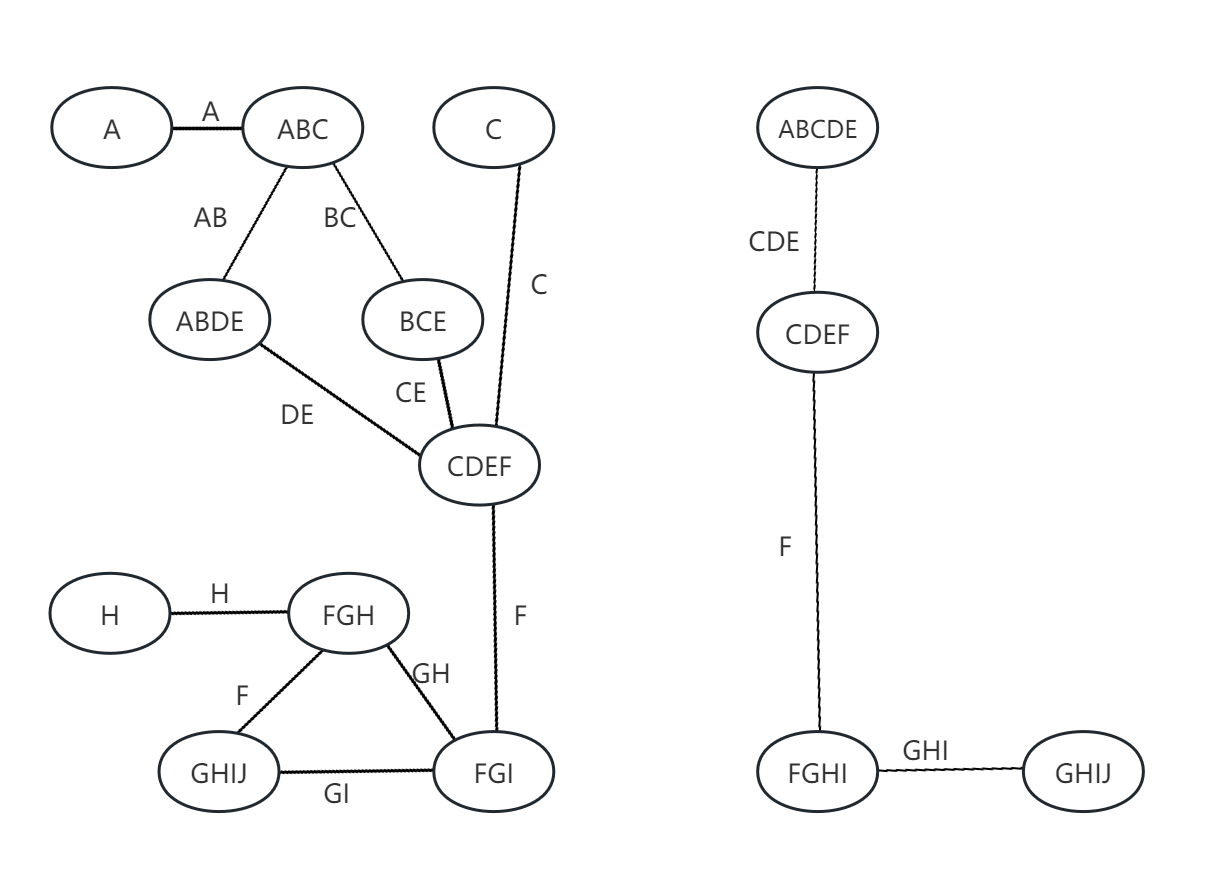
\includegraphics[width=0.6\textwidth]{png/JG.png}
\caption{In the picture A,B,C... representing variables(Clause nodes are hidden, and clause nodes 
cannot appear on edges),the shared variables between the two clusters act as edge-lable. the same 
factor graph can be decomposed into different tree decomposition forms, such as low tree-width on the 
left but with poor precision and high tree-width on the right with high complexity but high precision.} 
\label{fig2}
\end{figure}
\subsection{Tree Decomposition and Attention}
The method of using attention to solve the satisfactibility problem has been shown to be effective in 
previous work, but its huge overhead makes it impossible to solve larger instances, assuming that the 
input is a CNF formula containing n variables and m clauses, the total graph attention needs to calculate 
the interaction of all node pairs in the space \(O((n+m)^2)\). In our model AEIN, the attention mechanism 
is applied to each cluster after decomposition by tree decomposition method, and the consumption is greatly 
reduced to \(O(k⋅w^2)\). The larger the scale of the case, the more significant our improvement.
In our work, we adopted three attention mechanisms to optimize the model, which are introduced in this section.
In the Attention mechanism, Attention(Q,K,V) is the core computing module used to dynamically weight 
aggregated information based on the interaction of Query, Key, and Value.In Scaled Dot-Product Attention 
defined as:
\begin{equation}
Attention(Q,K,V)=softmax(\frac{QK^T}{\sqrt{d_k}})V
\end{equation}
\subsubsection{Hierarchical attention mechanism}
The core purpose of Hierarchical Attention mechanisms in AEIN models is to efficiently capture local and 
global dependencies in graph structures through hierarchical, granular information aggregation, thereby 
reducing computational overhead while improving the model's ability to reason about complex constraints.\\

Local: The microscopic interaction between the attention-focused variable and the clause within the cluster 
(such as the polarity conflict of variables within the clause).
The contribution weights of \(x_1\) and \(x_2\) to \(\phi_1\) are calculated in the cluster 
\(C_1=\{x_1,x_2,\phi_1=(x_1\bigvee ¬x_2)\}\) so that high weights are assigned to variable assignments 
that are more likely to satisfy the clause;\\

Variables and clauses inside cluster \(C\) calculate attention weights:\\
\begin{equation}
\alpha_{intra}=LekyReLU(\frac{(W_Qh_i)^T(W_Kh_j)}{\sqrt{d}}),\ \ \forall x_i,x_j\in C_k
\end{equation}\\
For variable node \(x_i\) and clause node \(\phi_j\) in cluster \(C\), the message passing formula is:
\begin{equation}
    m_{x_i\rightarrow \phi_j}^{(k)}=\alpha_{intra}\cdot \prod_{u\in \mathcal N(x_i)\textbackslash \phi_j}
    m_{u\rightarrow x_i}^{(k)}
\end{equation}
\begin{equation}
     m_{\phi_j\rightarrow x_i}^{(k)}=\alpha_{intra}\cdot\sum_{C_k \textbackslash \{x_i\}}
     \phi_j(C_k)\cdot\prod_{v\in \mathcal{N}(\phi_j)\textbackslash x_i}m_{v\rightarrow \phi_j}^{(k)}
\end{equation}
Update clause and variable feature:\\
\begin{equation}
h'_j=\sum_{x_i\in C_k}\alpha_{intra}W_Vh_i
\end{equation}\\
Global: Inter-cluster attention transmits macro-constraints across clusters (such as consistency of 
assignment of distant variables) through shared variables.
If clusters \(C_1\) and \(C_2\) share the variable \(x_2\), then attention determines the influence 
of \(C_1\) and \(C_2\) on the assignment of \(x_2\). If \(C_1\) and \(C_2\) tend to conflict on \(x_2\), 
the attention weight automatically adjusts the message passing intensity.
Calculate the attention weight of clusters \(C_1\)  to \(C_2\)  by passing cross-cluster messages 
through shared variables:
\begin{equation}
\alpha_{inter}=LekyReLU(\frac{(W_Qh_{C_1})^T(W_Kh_{C_2})}{\sqrt{d}})
\end{equation}
For adjacent clusters \(C_1\) and \(C_2\)(shared variable \(S_{12}=C_1\bigcap C_2\)), the inter cluster 
message is:
\begin{equation}
    m_{C_1\rightarrow C_2}(S_{12})=\alpha_{inter}\cdot\sum_{C_1\textbackslash 
    S_{12}}(\phi_1(C_1)\cdot\prod_{k\in ne(C_1)\textbackslash C_2}m_{k\rightarrow C_1})
\end{equation}
Update shared variable characteristics:
\begin{equation}
h'_x=h_x^{(C_1)}+\alpha_{inter}W_Vh_x^{(C_2)}
\end{equation}
\subsubsection{Dynamic attention mechanism}
The dynamic attention mechanism in AEIN model is realized by dynamically adjusting the number of 
attention heads to balance the performance of the model in different training stages and different 
complexity clauses. Start training with fewer attentional heads, quickly capture simple patterns 
(such as explicit constraints of short clauses), avoid overfitting, gradually increase the number of 
heads as the number of training steps increases to improve expressiveness, and deal with complex 
clauses (such as long chain dependencies) 
\begin{equation}
H(t)=min(H_{max},H_{init}+\lfloor\frac{t}{T}\rfloor)
\end{equation}
Assign a learnable weight to each attentional head \(\lambda_h\), dynamically adjusting its contribution:
\begin{equation}
\alpha_{dy}=\frac{1}{H(t)}\sum_{h=1}^H(t) \lambda_h Attention(Q,K,V)
\end{equation}
When \(\lambda_h\) is updated by gradient descent, the weight of important heads increases and 
the weight of redundant heads approaches 0.
This design allows AEIN to efficiently handle highly heterogeneous clause structures in \#SAT problems 
while maintaining low computational costs.

\subsubsection{Constraint-Aware Mechanism}
In AEIN, the central role of the Constraint-Aware Mechanism is to explicitly guide the model to 
preferentially satisfy clause constraints in the CNF formula, thus more efficiently approaching the 
correct model count. The realization method combines attention weight adjustment and loss function 
regularization.For each clause \(C_i\), define its satisfaction score \(s_i\):
\begin{equation}
s_i=sigmoid(\sum_{x_j\in \phi_i}(2b_j(x_j)-1)polarity(x_j,\phi_i))
\end{equation}
where, \(b_j(x_j)\) is  the current assignment probability of \(x_j\) ;  \(polarity(x_j,\phi_i)\) 
represents the polarity of \(x_j\) in the clause \(\phi_i\) .
\(s_i\in (0,1)\), where the closer to 1 means that the clause \(\phi_i\) is more likely to be 
satisfied.Add the following regularization terms to the loss function:
\begin{equation}
\mathcal L_{cons}=-\delta  \sum_{i=1}^mlns_i,
\end{equation}
Combining the RMSE and the constrained aware regularization term, the total loss function is:
\begin{equation}
\mathcal L_{total}=\mathcal L_{RMSE}+\mathcal L_{cons}
\end{equation}
The constraint awareness mechanism acts on the other mechanisms, implicitly adjusting the message 
passing process, using \(s_i\) weighted messages when propagating within and between clusters:
\begin{equation}
\alpha_{intra}=LekyReLU(\frac{(W_qh_i)^T(W_kh_j)+\gamma s_i}{\sqrt{d}})
\end{equation}
\subsection{\#SAT}
In join-graph, we need to modify the Bethe formula to fit the specific structure of the join-graph:
\begin{equation}
   F_{Bethe-Join}=\sum_\alpha [H(b_{C_\alpha})-\sum_{v\in C_\alpha}(d_v^\alpha-1)H(b_v)]
\end{equation}
\(H(b_{C_\alpha})\) is the joint distribution entropy of variables and clauses within cluster \(C_\alpha\), 
\(H(b_v)\) is the entropy of the local variable, are the \(GAT1\) and \(GAT2\) outputs respectively, 
which are used as the input of the MLP layer after the pooling operation. the goal of the MLP is to 
approximate \(F_{Bethe-Join}\) by  the hierarchical structure of the join-graph.Its inputs and specific 
implementation are as follows:
\begin{equation}
    h_{C_\alpha}=[H(b_{C_\alpha}), \sum_{v\in C_\alpha}(d_v^\alpha-1)H(b_v)], h_G=\frac{1}
    {\mid{C_\alpha}\mid}\sum_\alpha h_{C_\alpha}
\end{equation}
\begin{equation}
   H(b_{C_\alpha})=GAT1(\frac{1}{ \mid C_\alpha\mid}\sum_{j\in C_\alpha}h_j), H(b_v)=GAT2(h_x)
\end{equation}

The MLP fits the following mappings:
\begin{equation}
    \hat{F}_{Bethe-Join}=W_2\cdot ReLU(W_1h_G+b_1)+b_2
\end{equation}
\( W_1\in\mathbb{R}^{d\times 2}, b_1\in \mathbb{R^d}\) is the MLP hidden layer parameter\
and the \(W_2\in\mathbb{R}^{1\times d} , b_2\in \mathbb{R}\) is the output layer parameter. 
By supervised ground truth logZ (precomputed by the exact method), the loss function is designed 
as follows \(\mathcal L_{total}\), finally, make a prediction:
\begin{equation}
    logZ\approx -\hat{F}_{Bethe-Join}=-MLP(h_G)
\end{equation

\section{Experimental Evaluation}
\subsection{Experiment Setup}
In all experiments, we set the feature dimension d = 64 and the number of message passing iterations T=5 for training. 
2GAT + MLP serial connection. The initial number of attention heads is four and is increased by one every 1000 steps 
until eight. We run all experiments on the server using a single NVIDIA A100 GPU and eight CPU cores.
We first follow the experiment settings in recent work NSNet. Specifically, we run experiments using the same subset 
of BIRD benchmark\cite{A19} , which contains eight categories arising from DQMR networks, grid networks, bit-blasted 
versions of SMTLIB benchmarks, and ISCAS89 combinatorial circuits. Each category has 20 to 150 CNF formulas, which we 
split into training/testing with a ratio of 70\%/30\%. Note that the BIRD benchmark is quite small and contains 
large-sized formulas with more than 10,000 variables and clauses, it challenges the generalization ability of our model. 
Besides evaluating in such a data-limited regime, we also conduct experiments on the SATLIB benchmark, an open-source 
dataset containing a broad range of CNF formulas collected from various distributions. To train our model effectively, 
we choose the distributions with at least 100 satisfiable instances, which include the following 5 categories: (1) uniform 
random 3-SAT on phase transition region (RND3SAT), (2) backbone-minimal random 3-SAT (BMS), (3) random 3-SAT with controlled
backbone size (CBS), (4) "Flat" graph coloring (GCP), and (5) "Morphed" graph coloring (SW-GCP). The whole dataset has 
46,200 SAT instances with the number of variables ranging from 100 to 600, and we split it into training/validation/testing 
sets with a ratio of 60\%/20\%/20\%. For both BIRD and SATLIB benchmarks, we ran the state-of-the-art exact \#SAT solver 
DSharp\cite{B7} with a time limit of 5,000 seconds to generate the ground truth labels. The instances where DSharp fails to 
finish within the time limit are discarded.

\subsection{Evaluation \& Baselines.}
Following BPNN and NSNet, we use the (1) root mean square error (RMSE) between the estimated log countings and ground truth 
as our evaluation metrics. We compare AEIN , the neural baseline BPNN and NSNet, and two state-of-the-art approximate model
counting solvers, ApproxMC3\cite{A19} and F2\cite{B8}. For ApproxMC3 and F2, we set a time limit of 5,000 seconds on each instance.

\subsection{Main Results}
\begin{figure}[htbp]
    \centering
    \begin{subfigure}{0.48\textwidth}
        \centering
        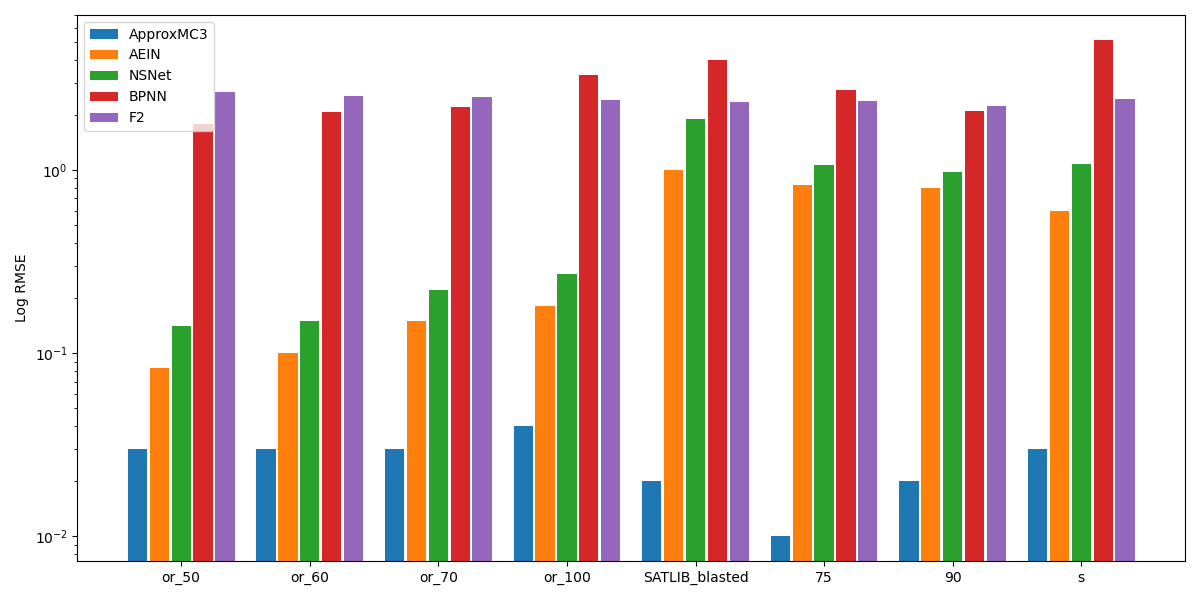
\includegraphics[width=\linewidth]{png/柱状图.png} % 图片1路径
        \caption{}
        \label{fig:sub1}
    \end{subfigure}
    \hfill % 水平填充间距
    \begin{subfigure}{0.48\textwidth}
        \centering
        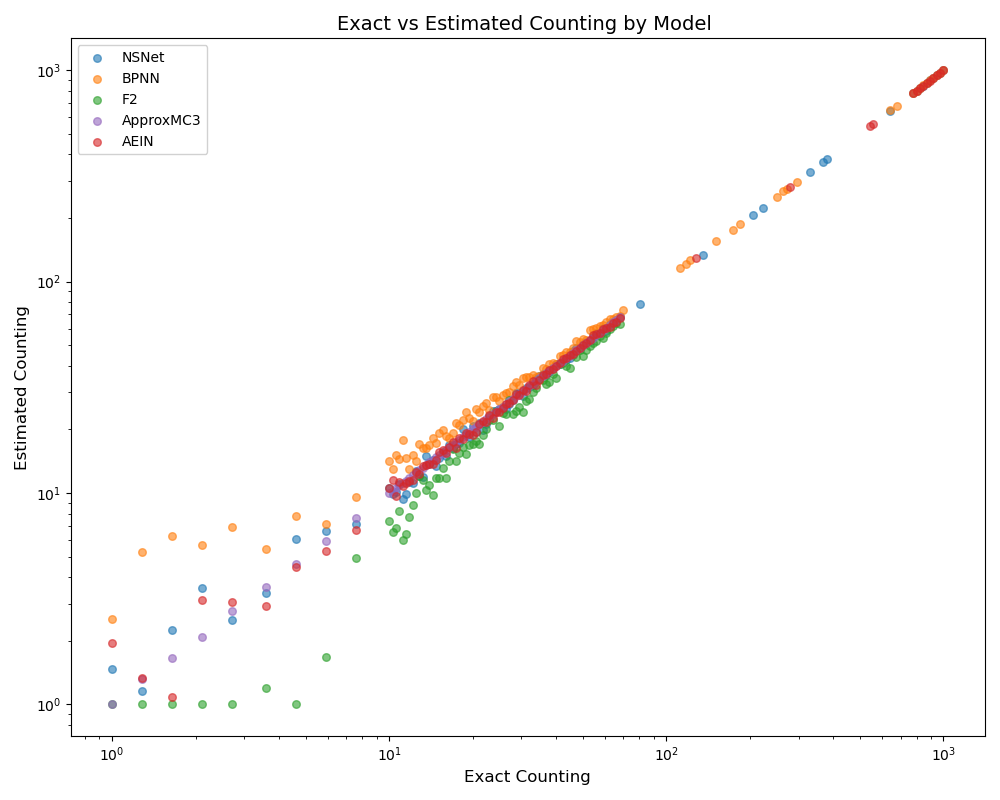
\includegraphics[width=\linewidth]{png/plot.png} % 图片2路径
        \caption{}
        \label{fig:sub2}
    \end{subfigure}
    \caption{(a) is RMSE between estimated log countings and ground truth for each solver on the BIRD benchmark;
    (b) is Scatter plot comparing the estimated log countings against the ground truth for each solver on the BIRD benchmark}
    \label{fig:total}
\end{figure}
As shown in Figure~\ref{fig:sub1}, AEIN can estimate tighter counts than NSNet, BPNN, and F2 in all categories of the BIRD benchmark. 
AEIN estimates are almost three times more accurate than F2 and BPNN. However, AEIN cannot compete with ApproxMC3.
Table 1 shows the detailed RMSE results for each solver on the SATLIB benchmark. All SATLIB datasets were generated manually and 
randomly, and the accuracy decreased compared to the BIRD dataset, but AEIN still achieved an advantage in all categories.
Figure~\ref{fig:sub2} shows the scatter plot. The estimated logarithmic count is compared to the ground truth for each solver on 
the BIRD benchmark. When the ground truth is less than \(e^{100}\), AEIN and ApproxMC3 can provide more accurate estimates than NSNet, 
F2 and BPNN in most cases. ApproxMC3 is unable to complete in 5000 seconds when the ground truth count exceeds \(e^{100}\), AEIN can 
still give a close approximation when the ground truth count exceeds \(e^{1000}\). This demonstrates the effectiveness of AEIN in solving 
difficult and large cases.

Table~\ref{tab1} shows the detailed RMSE results for each solver on the SATLIB benchmark. The data for the BIRD benchmark is collected 
from many real-world model counting applications that may share many common logical structures to learn, whereas instances in the SATLIB 
benchmark are randomly generated, making it difficult for AEIN to exploit common features. Despite this, AEIN still outperforms NSNet 
and F2 in most categories.

\begin{table}[htbp] 
  \centering  
  \caption{RMSE between estimated log countings and ground truth for each solver on the SATLIB benchmark.}  
  \begin{tabular}{ccclll}  
    \toprule
    Method& RND3SAT& BMS & CBS& GCP&SW-GCP\\  
    \midrule
    F2& 2.13& 2.42& 2.37& 2.40&2.66\\  
    NSNet& 1.57& 2.45& 1.68& 2.14&1.37\\  
    AEIN& \textbf{1.15}& \textbf{1.66}& \textbf{1.20}& \textbf{1.96}&\textbf{0.96}\\  
    \bottomrule
  \end{tabular}
  \label{tab1}  
\end{table}\\
\begin{table}[htbp] 
  \centering  
  \caption{Ablation experiments of the AEIN model on three refinements.}  
  \begin{tabular}{ccclll}  
    \toprule
    Method& RMSE& Head utilization(\%)& Training time/convergence\\ 
    \midrule
    GAT& 1.33& 100& 185.155\\  
    GAT-H& 1.26& 100& 153.499\\  
    GAT-HC& 1.19& 100& 170.164\\
    \centering  
    GAT-HCD& 1.16& 62.5& 113.165\\  
    \bottomrule
  \end{tabular}
  \label{tab2}  
\end{table}\\
To prove that the three attention mechanisms of our AEIN model are effective, Table~\ref{tab2} shows its ablation experiments 
with RMSE, attention head utilization and training time as evaluation metrics. Experiments show that the three attention mechanisms 
all play a positive role in the model. Among them, the hierarchical attention mechanism and constraint perception mechanism greatly 
improve the accuracy of the model, and the dynamic attention mechanism reduces the redundant attention head over time, avoids more 
calculations, reduces the training time and improves the efficiency of the model.

Traditional model counting methods include: model counter based on search,for example, 
the DPLL process. These algorithms usually produce accurate counts, but can only handle 
relatively small formulas. (2006), Thurley uses new component caching techniques and 
decision heuristics to propose the SharpSAT solver\cite{B9}; Model counter based on 
compilation, knowledge representation (i.e. target language), the model number can be 
efficiently calculated and queried in the new target language.  (2021)Lai et al. proposed 
a new knowledge representation method CCDD\cite{A21} incorporating literal equivalence, 
and proposed a new model counter ExactMC\cite{A22} based on CCDD; Model counter based 
on elimination, This method does not solve the model number by eliminating all variables 
at one time, but uses the idea of dynamic programming to constantly find the variables 
that can be eliminated in the process of solving, and finally gets the model number. Such 
solvers include ADDMC\cite{A20} and DPMC\cite{A23} solvers proposed by Dudek et al. (2020). 
The former completes the elimination process by algebraic decision graph and heuristic 
method, and the latter uses the idea of tree decomposition to construct Join-Tree for 
elimination.\\
As neural networks have demonstrated superior learning capabilities, the use of data-driven 
approaches to the \#SAT problem has become a new direction. Early works like NeuroSAT\cite{A24} 
demonstrated that GNNs could learn to predict satisfiability by message passing on  variable 
clause bipartite graphs. (2020)Sebastian J et al. 's Neural heuristics\cite{A25} uses neural 
graph networks with message passing architectures and attention mechanisms to enhance the 
branch heuristics of two SAT solving algorithms. (2020)J Kuck et al. combined message passing 
algorithm with neural network to get BPNN architecture, which can learn neural network to 
olve combinatorial optimization and decision problems.Compared with the most advanced manual 
design method, BPNN architecture can be developed. BPNN can calculate speeds up to 100 times 
higher. (2022)G averi et al. 's BPGAT\cite{A26} serves as an approximate model counter to the 
CNF formula by extending the BPNN architecture and introducing an attention mechanism. 
(2023)Yifan Zhang proposed and implemented BPMC\cite{M1}, a neural network solver based on 
belief propagation, which can give the approximate model calculation value of the instance 
in a very short time, and the solution time is basically not affected by the size of the 
instance.

In this work, we propose a neural framework for solving the satisfiability problem. 
Our framework combines tree decomposition and GAT, includes IJGP in the latent space, 
and performs partition function estimation to solve \#SAT. Experimental evaluation 
on synthetic datasets and existing benchmarks shows that our approach significantly 
outperforms NSNet and other neural baselines and achieves competitive results compared 
to state-of-the-art solvers.


\bibliographystyle{plain}
\bibliography{references}
\end{document}
